\documentclass[12pt,a4paper,twoside]{book}


% =================================================
% CORE PACKAGES
% =================================================
\usepackage[margin=1.2in]{geometry}
\usepackage{graphicx}
\usepackage{amsmath}
\usepackage{subcaption}
\usepackage{float}
\usepackage{siunitx}
\usepackage{chemformula}
\usepackage[version=4]{mhchem} % ONLY this, not twice
\usepackage{titling}
\usepackage{xcolor}
\usepackage{fancyhdr}
\usepackage{booktabs}
\usepackage{pdfpages}
\usepackage{makecell}

% =================================================
% TYPOGRAPHY
% =================================================
\usepackage{microtype}
\usepackage{newunicodechar}
\newunicodechar{−}{-}

% =================================================
% HYPERLINKS
% =================================================
\usepackage{hyperref}
\usepackage{xurl}

% =================================================
% BIBLIOGRAPHY
% =================================================
\usepackage[backend=biber,style=phys]{biblatex}

\addbibresource{Bibliography/references_m.bib}

% =================================================
% ABBREVIATIONS
% =================================================
\usepackage[acronym]{glossaries}
\makeglossaries
\newacronym{API}{API}{application programming interface}
\newacronym{ATI}{ATI}{above-threshold ionization}

\newacronym{BBO}{BBO}{beta-barium borate}
\newacronym{CAMP}{CAMP}{CFEL-ASG Multi-Purpose instrument}
\newacronym{HOMO}{HOMO}{highest occupied molecular orbital}
\newacronym{NIR}{NIR}{near-infrared}
\newacronym{UV}{UV}{ultraviolet}
\newacronym{CEI}{CEI}{Coulomb explosion imaging}
\newacronym{PES}{PES}{potential-energy surface}
\newacronym{IP}{IP}{ionization potential}




















% =================================================
% PAGE GEOMETRY (INNER/OUTER)
% =================================================
\newgeometry{
  top = 0.75in,
  bottom = 0.75in,
  outer = 0.75in,
  inner = 1.1in
}

% =================================================
% HYPERREF SETUP
% =================================================
% Acronyms + internal links: BLACK
% Citations: BLUE
% URLs: RED
\hypersetup{
  colorlinks=true,
  linkcolor=blue,
  citecolor=blue,
  urlcolor=red
}

% =================================================
% HEADER / FOOTER STYLE
% =================================================
\renewcommand{\chaptermark}[1]{%
  \markboth{\textcolor{blue}{\chaptername\ \thechapter.\ #1}}{}%
}
\renewcommand{\sectionmark}[1]{%
  \markright{\textcolor{blue}{\thesection\ #1}}%
}

\fancypagestyle{mainstyle}{
  \fancyhf{}
  \renewcommand{\headrulewidth}{0.4pt}
  \renewcommand{\footrulewidth}{0pt}
  \fancyhead[LE,RO]{\bfseries\thepage}
  \fancyhead[LO]{\leftmark}
  \fancyhead[RE]{\rightmark}
}



% =================================================
% DOCUMENT
% =================================================
\begin{document}

% -----------------
% FRONT MATTER
% -----------------
\frontmatter
\pagestyle{empty}

\begin{titlepage}
\thispagestyle{empty}
\centering
\bfseries

\vspace*{2cm}

{\LARGE
Thesis Title
\par}

\vspace{2.5cm}

{\Large
Dissertation\\
zur Erlangung des Doktorgrades\\
an der Fakultät für Mathematik, Informatik und Naturwissenschaften\\[0.5
cm]
Fachbereich Physik\\
der Universität Hamburg
}

\vspace{2cm}

{\Large
vorgelegt von\\[0.3cm]
XXXX Kumar
\par}

\vspace{2cm}

{\Large
Hamburg\\
20XX
\par}

\vspace{2cm}



\end{titlepage}




\thispagestyle{empty}




%Second page for referee
%\noindent\hrulefill % Horizontal line across the page
\clearpage
\thispagestyle{empty}

\vspace*{10cm}

\noindent
\begin{tabular}{l@{\hspace{2.5cm}}l}
\textbf{Gutachter/innen der Dissertation:} & Prof.\ Dr.\ XXXX XXXX \\
                                           & Prof.\ Dr.\ XXXX XXXX \\
                                          
                                     
\end{tabular}

\vspace{1.5cm}

\noindent
\begin{tabular}{l l}
\textbf{Zusammensetzung der Pr\"ufungskommission:} & Prof.\ Dr.\ XXXXX XXXXX \\[0.3cm]
                                                   & Prof.\ Dr.\ XXXX XXXX \\[0.3cm]
                                                   & Prof. Dr.\ XXXX XXXX \\[0.3cm]
                                                   & Prof.\ Dr.\ XXXX XXXX \\[0.3cm]
                                                   & Prof.\ Dr.\ XXXX XXXX \\
\end{tabular}

\vspace{1.5cm}

\noindent
\begin{tabular}{l}
\textbf{Vorsitzender des Pr\"ufungsausschusses:} Prof.\ Dr.\ XXXX XXXX \\[0.5cm]
\textbf{Datum der Disputation:} XX.XX.2026 \\[0.5cm]
\textbf{Vorsitzender des Fach-Promotionsausschusses PHYSIK:} Prof.\ Dr.\ Johannes Haller\ \\[0.5cm]
\textbf{Leiter des Fachbereichs PHYSIK:} Prof.\ Dr.\ Markus Drescher \\[0.5cm]
\textbf{Dekan der Fakult\"at MIN:} Prof.\ Dr.-Ing.\ Norbert Ritter
\end{tabular}

%\clearpage
%\end{document}

\clearpage
\thispagestyle{empty}

\vspace*{\fill}

\begin{center}
\begin{minipage}{0.7\textwidth}
\centering
\textit{This work is dedicated to .........}
\end{minipage}
\end{center}

\vspace*{\fill}

\clearpage

% Abstract (EN)
\vspace*{\fill}
\section*{\Huge\bfseries Abstract}
\vspace{0.2cm}
Abstract of thesis in English..

\vspace*{\fill}

% Abstract (DE) 
\newpage
\section*{\Huge\bfseries Zusammenfassung}
Abstract of thesis in German.







































% TOC and glossary
\pagestyle{plain}
\tableofcontents

\printglossary[type=\acronymtype, title={List of Abbreviations}]

% -----------------
% MAIN MATTER
% -----------------
\mainmatter
\pagestyle{mainstyle}

\chapter{Introduction}
\label{chap:introduction}

This chapter introduces the research topic, outlines the motivation and objectives of the study, and provides an overview of the thesis structure \cite{atia-tul-noor_sub-50_2024}.

\section{Background}
Brief description of the research area and its context.

\section{Problem Statement}
Description of the research problem or gap addressed by the study. The \gls{IP} of X atom is x eV.

\section{Research Objectives}
Presentation of the main objectives and scope of the research.

\section{Thesis Organization}
Overview of the remaining chapters of the thesis.

\chapter{Theoretical Background}
\label{chap:theory}

This chapter presents the theoretical foundations and key concepts relevant to this research. These provide the necessary background for understanding the work presented in the following chapters.

\section{Overview}
Brief introduction to the theoretical background covered in this chapter.

\subsection{Fundamental Concepts}
Description of the core concepts and terminology relevant to the research.

\subsection{Related Theories}
Overview of the theories, models, or frameworks that underpin the study.




\chapter{Experimental Techniques}
\label{chap:experimental_techniques}

This chapter describes the experimental methods, techniques, instruments, and procedures employed in this research.

\section{Introduction}
Overview of the experimental approaches and methodologies used in the study.

\section{Materials and Methods}
Description of the materials, samples, and experimental procedures.

\subsection{Materials}
Details of the materials or samples used.

\subsection{Experimental Procedure}
Description of the methodology and workflow.

\section{Instrumentation}
Overview of the equipment, instruments, and measurement techniques employed.

\section{Data Collection and Analysis}
Description of data acquisition, processing, and analysis methods.

\input{Chapter/Result1/Result1}
\input{Chapter/Result2/Result2}
\chapter{Result3}
\label{chapter:result3}

\section{Introduction}
The chapter focuses on presenting the results, while detailed interpretation and discussion are provided in the subsequent chapter.

\section{Experimental Setup}
Briefly describe the experimental conditions.

\section{Results and Analysis}
Present the main findings of the study. 

\subsection{Result Category 1}
Present results using tables, figures, and descriptive analysis.

\subsection{Result Category 2}
Present additional findings and comparative analyses.

\section{Summary}
This chapter presented the experimental results and their preliminary analysis. 
\chapter{Summary and Outlook}
\label{chap:summary}

This chapter summarizes the main findings and contributions of the research and discusses potential directions for future work.

\section{Summary}
Overview of the research objectives, methodology, and key outcomes.

\section{Outlook}
Discussion of future research opportunities, extensions, and potential applications.




%%%%%%%%%%%%% back page %%%%%%%%%%%%%%%%%%%%%%%


% -----------------
% APPENDICES
% -----------------
\clearpage
\appendix
\pagestyle{plain}
\appendix

\chapter{Appendix A}
\label{app:a}

Supplementary material related to the research presented in this thesis.

\section{Additional Information}
Supporting details, derivations, figures, tables, or data.

\chapter{Appendix B}
\label{app:b}

Additional technical information and supplementary results.

\section{Supplementary Methods}
Further details of methodologies, procedures, or analyses not included in the main text.


% -----------------
% BIBLIOGRAPHY
% -----------------
\clearpage
\begingroup
\sloppy
\printbibliography
\endgroup

% -----------------
% PUBLICATIONS
% -----------------
\clearpage
\chapter*{List of Publications}
\addcontentsline{toc}{chapter}{List of Publications}

Parts of this work have been published in the following peer-reviewed journal articles:

\begin{enumerate}
    \item XXXX

\end{enumerate}


\footnotetext[1]{These authors contributed equally to this work.}


% -----------------
% DECLARATION
% -----------------
\clearpage
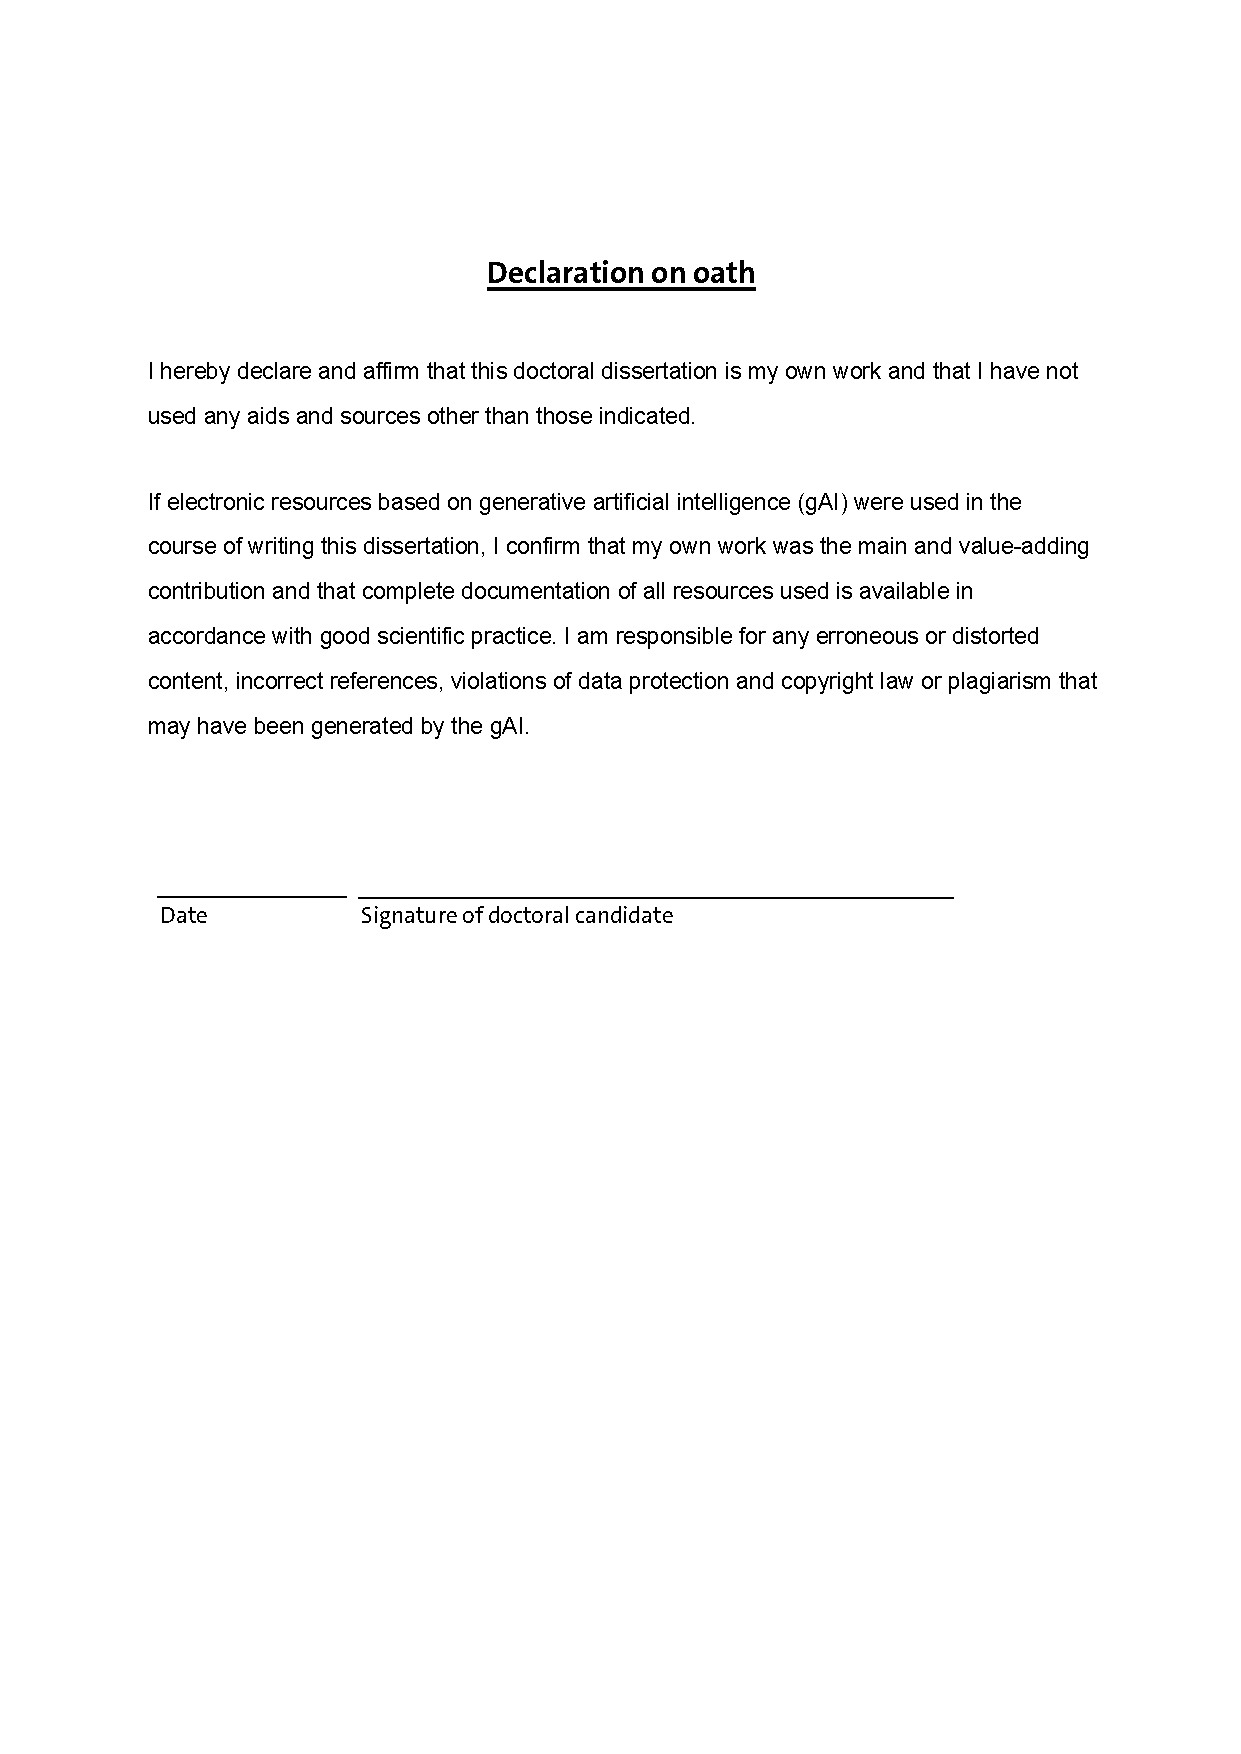
\includepdf[pages=-, pagecommand={}, fitpaper=true]{Back_Page/Declaration/oath.pdf}

% -----------------
% ACKNOWLEDGMENTS
% -----------------
\clearpage
\input{Back_Page/acknowledgment}

\end{document}
